\chapter{Theory of Clouds and Radiation}%("Theory of ...."?)
\label{chap:theory}
In this chapter, a brief overview of clouds in the Arctic, with focus on stratus, is presented first. Followed by how cloud properties can influence radiation. Last in this chapter, a section on aerosol-cloud interactions is included.

%How clouds scatter and absorb SW and LW radiation.
%Explain something about blackbodies, clouds and blackbodies?

\section{Arctic clouds}% Arctic stratus??
%\section{Clouds} \subsection{The basics} \subsection{The Arctic}
The Arctic cloud cover is dominated by low clouds, and the largest amounts of low stratus clouds are over the open oceans~\citep{Klein1993}. %The Arctic is the only region where the season of maximum stratus does not correspond to the season of greatest lower troposphere static stability~\citep{Klein1993}, which could be due to lack of evaporation during the cold winter months.
 According to~\citet{Klein1993} stratus in the Arctic basin peaks during summer at nearly 62\%, while during the winter season the stratus only accounts for 18\% of the cloud cover. This leads them to conclude that the seasonal cycle of stratus in the Arctic is driven by the temperature cycle, thereby moisture content in the atmosphere, rather than the static stability.
%(, as opposed to other areas.)
%Are there any typical cloud properties special to the arctic? CURRY!

Low clouds have bases below 2000~m. Stratus (St) are layered clouds that form when extensive areas of stable air are lifted. Stratus clouds are normally between 0.5 and 1~km thick, whereas they can be several km wide~\citep{Aguado2010}.

The air in the Arctic is very stable in winter (polar night), and clean since there are not many sources for pollution. In Autumn the sea ice extent reaches a minimum after the summer melting and leaves open water to influence low clouds and their properties.  Some of the cloud radiative properties are presented in the next section.

\begin{figure}
\centering
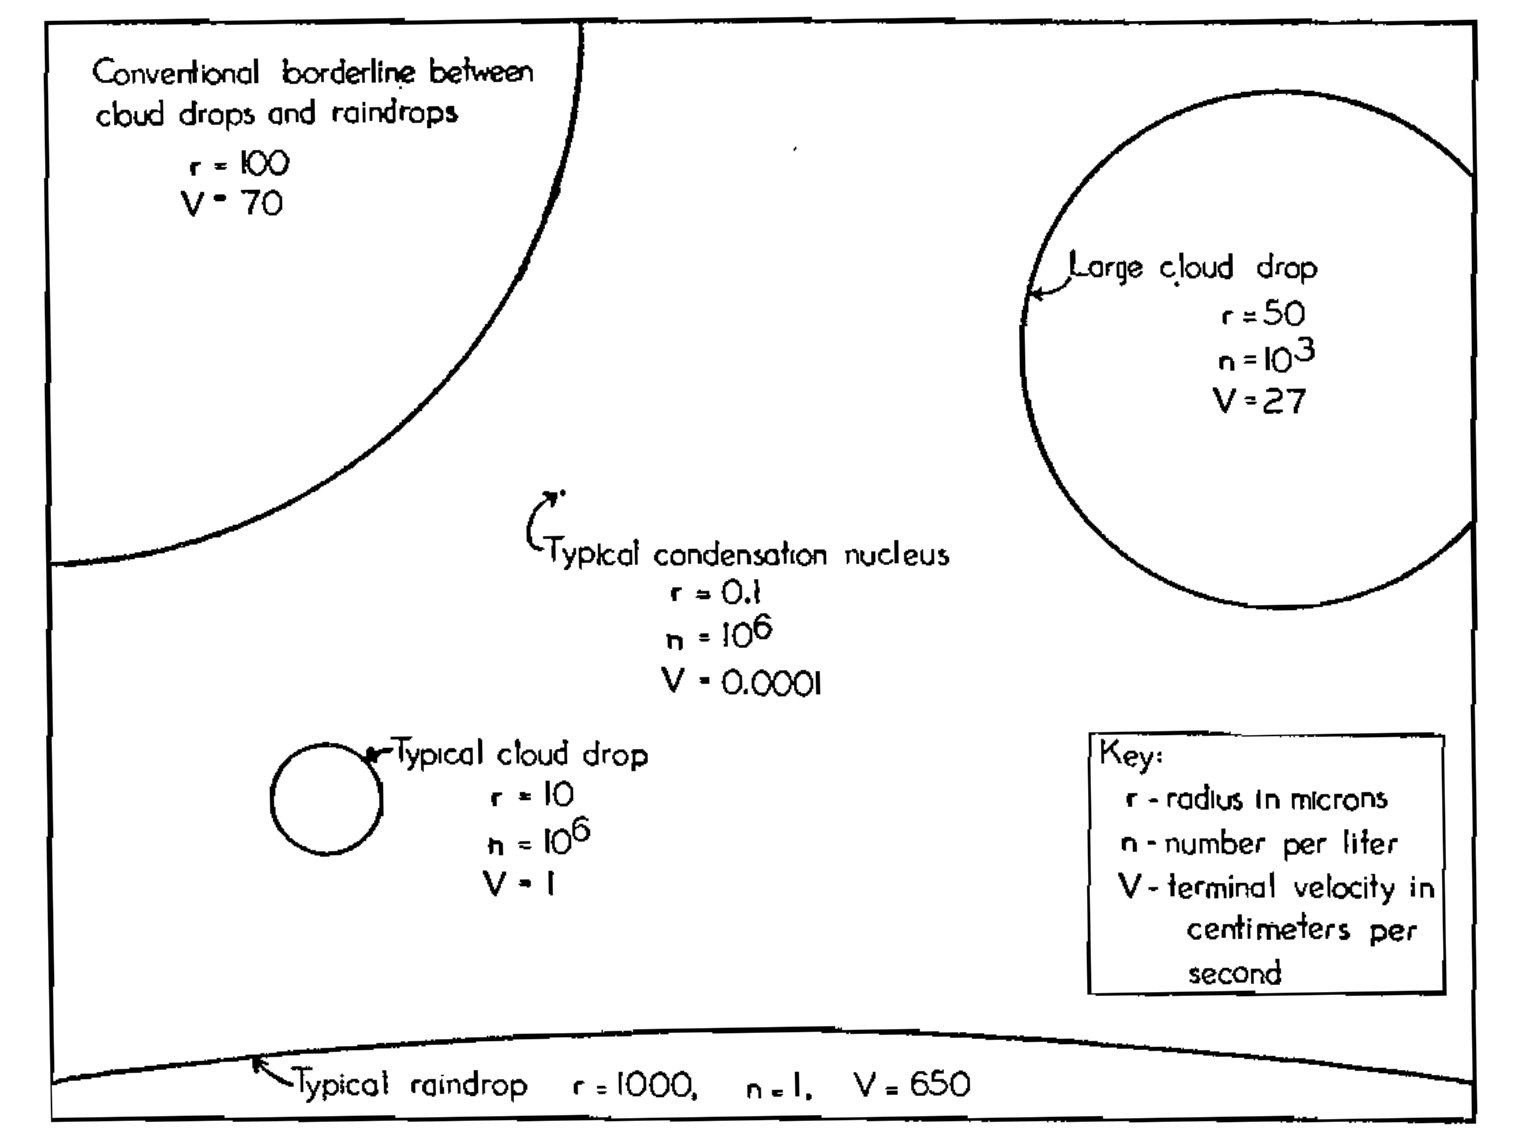
\includegraphics[width=0.85\textwidth]{theory/dropletsize.png}
\caption{Size of CCN, typical cloud droplet, large cloud droplet, borderline between cloud droplets and raindrops and typical size of raindrop.% Adapted
 From~\citep{McDonald1958}.}
\label{fig:dropletsize}
\end{figure}

\section{Cloud effects on radiation}
Is this where I should include the part about heating (not cooling) effect of low cloud in the Arctic, as opposed to global mean which is cooling?

As mentioned in Chapter~\ref{chap:introduction} there is no solar radiation to reflect during winter and the polar night in the Arctic, whereas in the summer the zenith angle is so high that even though there is sunlight 24 hours a day the cooling effect in summer does not average out the heating effect the clouds have in winter. A high zenith angle, means that the radiation has to travel through more atmosphere, which gives a higher optical depth and stronger depletion of the radiation beam. Consequently, the low clouds' ability to absorb and emit terrestrial radiation dominates over their reflective effect on the solar radiation.

The cloud microphysical properties that determine the cloud radiative properties include: the amount of condensed water, the size and shape of the cloud particles, and the phase of the particles/and if the particles are liquid or ice~\citep{Curry1996}.
\subsection{The Cloud -- a gray body}
Stefan–Boltzmanns law states that the flux density emitted by a blackbody is proportional to the fourth power of the absolute temperature~\citep{Liou2002}. 
\begin{equation}
F = \epsilon_{\lambda} \sigma T^4
\end{equation}
where $\epsilon_{\lambda} = 1$ is the emissivity for a blackbody at wavelength $\lambda$. $F [W~m^{-2}]$ is the flux density emitted  by the body, and $\sigma = 5.67\cdot 10^{-8} Jm^{-2}sec^{-1}deg^{-4}$ is the Stefan–Boltzmann constant. A blackbody both absorbs and emits at maximum, and the ratio of absorption and emission to the maximum is given by the absorptivity, $\alpha_{\lambda}$, and the emissivity, $\epsilon_{\lambda}$, for wavelength $\lambda$. Kirchoff's law states that the absorptivity and emissitivty for a medium are equal for each wavelength: $\alpha_{\lambda} = \epsilon_{\lambda}$. Kirchoff's law is only applicable at local thermodynamic equilibrium in the lower 60-70~km of the atmosphere. Since this study focuses on the lowest 2-3~km of the troposphere, the law is applicable.

A cloud can be defined as a a gray body, which means that $\alpha_{\lambda}$and $\epsilon_{\lambda}$ are not maximum, $\alpha_{\lambda}=\epsilon_{\lambda}<1$~\citep{Liou2002}. %The cloud LW? emissivity is given by
%\begin{equation}
%\epsilon_{\lambda} = @fill in
%\end{equation}

Since the gray body does not have maximum absorption, some of the radiation flux incident on the medium must be reflected. For a cloud this is represented by the cloud albedo, given by
\begin{equation}
A = \frac{(1-g)\tau}{1+(1-g)\tau} = \frac{1-g}{\frac{1}{\tau}+(1-g)}
\end{equation}
%should this equation have a label? yes@

So now I have to explain about the asymmetry factor (g) and the single scattering albedo ($\tilde{\omega}$) which has been approximated to one for this equation to be valid for the cloud albedo. According to Twomey, g=0.8 or 0.9 for warm clouds. g=1 is pure forward scattering and g=-1 is pure back-scattering. The asymmetry factor gives the direction of the scattered radiation. $g=\overline{\cos \theta}$ where $\theta$ is the scattering angle. A power-averaged value of the cosine of the scattering angle~\citep{Twomey1974}.

\subsection{Cloud optical depth}
Cloud optical depth or cloud optical thickness, $\tau$, is a measure of the cumulative depletion that a beam of radiation directed straight downward (zenith angle $\theta = 0$) would experience in passing through a defined cloud layer. The cloud optical depth is given by~\citep{Twomey1977}
\begin{equation}
\tau = \int_0^h k_{E}dz = \pi \int_0^h \int_0^{\infty}r^2Q_E(r/\lambda)n(r,z)drdz
\end{equation}
at height z above cloud base for a cloud of depth $h$, containing $n(r)dr$ drops with radius in the interval ($r, r + dr$) per cubic centimeter. 
$Q_E(r/\lambda$ is the extinction efficiency and $k_{E}$ is the extinction coefficient~\citep{Twomey1977}. In the visible, for $\lambda<<r$, $Q_E\approx 2$ is a good approximation~\citep{Liou2002}, and we get the simpler expression
\begin{equation}
\tau = 2\pi N r_e^2h
\end{equation}
where it is assumed that the cloud droplet radius can be approximated by the effective radius, $r_e$.


\subsection{Cloud droplet effective radius}
The cloud droplet effective radius determines important radiative properties of a cloud, cloud albedo ($A$) and cloud emissivity ($\epsilon$)~\citep{Hansen1974}, and is therefore of particular interest.

The cloud droplet effective radius is a weighted mean of the size distribution of cloud droplets. The effective radius may be written
\begin{equation}
r_e = \frac{\int r^3 n(r) dr}{\int r^2 n(r) dr}
\end{equation}
where $r_e$ is the effective radius.

%It is obvious from equations for $A$ and $\epsilon$ that a when $r_e$ is small - the albedo increases, and when it is larger the cloud albedo decreases. What about emissivity??

%How do clouds reflect radiation? What is the effect of more water? Or more ice? What about the droplet size? (effective radius)\\
%How do clouds absorb and emit radiation? Effect of more or less water or ice? Droplet size?    INCLUDE RADIATION EQUATION!

%Ice is more effective in reflecting SW than water. Snow has a higher albedo than rain. Is there any use in presenting some albedo values for water, snow, ice? Or open water versus sea ice? New ice versus old sea ice?

\subsection{Liquid Water Content and Path}
 The amount of condensed water can be expressed by the liquid water content (LWC) in the cloud, often presented with units g~m$^{-3}$ and is proportional to the cloud droplet number concentration. From~\citet{Rogers1989} we can express the number of droplets with radius $r$ by
\begin{equation}
N = \int n(r) dr
\end{equation}
where $N$ is the cloud droplet number concentration (cm$^{-3}$), and $n(r)$ is the number of droplets with radius $r$. When we use the median volume radius, $\overline{r}$ ($\mu m$), the LWC can be written
\begin{eqnarray}
LWC &=& \int \rho_L \frac{4}{3} \pi r^3 n(r) dr\\
&=& \frac{4}{3} \pi \rho_L \int r^3 n(r) dr\\
&=& \frac{4}{3} \pi \rho_L \overline{r}^3 \int n(r) dr\\
&=& \frac{4}{3} \pi \rho_L \overline{r}^3 N 
\end{eqnarray}
where the last equation shows the proportionality of LWC to the cloud droplet number concentration $N$, and to $\overline{r}$. $\rho_L$ is the density of liquid water.

Another common measure of condensed water is the liquid water path (LWP).
If the LWC is integrated over a column, from the base to the top, it gives the LWP of that column.
\begin{equation}
LWP = \int_{base}^{top} LWC dz
\end{equation}
The LWP is the column of liquid water in a cloud and is usually expressed by $g~m^{-2}$.

%How does this influence the radiation???!!
A higher LWC or LWP increases the reflectivity of the cloud, and thereby reduces the SW radiation reaching the surface.


\section{Aerosols and clouds}%Aerosols and clouds som tittel??
For low clouds to form there must be available aerosols. Aerosols act as cloud condensation nuclei (CCN) by letting water vapor condense on them. This is how a cloud droplet is formed. For an ice particle to be present in a low cloud, an ice nuclei (IN) and low temperatures %(-5 to -20$^o$C)@? 
are necessary. If an IN hits a cloud droplet with temperature below zero, a super-cooled droplet, the droplet will freeze.

Aerosols have a direct effect on the climate by scattering and absorbing SW radiation, and scattering, absorbing and emitting LW radiation.% acting as CCNs og INs. elaborate?
They also have an effect on climate through clouds, an indirect effect. The amount of CCNs and INs available affect the properties of the clouds in the area. There are two known indirect effects that aerosols have on radiation, through clouds. The first indirect effect was proposed by~\citet{Twomey1974} and is often referred to as the Twomey effect. The second indirect effect was proposed by~\citet{Albrecht1989} and is also known as the lifetime effect.


\subsection{The first indirect effect}% (Maybe just call it all indirect effects and refer to Lohmann and Feichter)
If there are few CCNs in an area, a cloud formed there would be a clean cloud with few, but large droplets and therefore have a low albedo and precipitate easily. If the area had high aerosol concentration, the cloud would be polluted and have more numerous but smaller droplet, which means it would have a higher albedo and precipitation would be suppressed. 
The first indirect effect, suggested by~\citet{Twomey1974}, describes the enhancement of cloud albedo as a consequence of an increase in aerosol content and thereby available CCNs.
By increasing droplet concentration and hence the optical thickness of a cloud, see equation 3.3%@give it a label?
, pollution acts to increase the reflectance of clouds. It is clear from equation 3.3 that if the droplet concentration is increased, so is the optical thickness of the cloud.

The cloud optical depth will change with changes in aerosol number concentrations and changes in clouds and their properties. For instance if a cloud has many small droplets, the cloud optical depth will be higher. Whereas fewer cloud droplets will yield a lower optical depth, resulting in more SW radiation reaching the ground —  having a warming effect on the area. 

(Include a figure showing the indirect effect)

\subsection{The second indirect effect}

The second indirect effect, or the cloud lifetime effect, suggests more numerous but smaller droplets reduce the precipitation efficiency and by that enhances the cloud lifetime and hence the cloud reflectivity~\citep{Albrecht1989}. This effect has been estimated to be roughly as large as the first indirect effect~\citep{Lohmann2005}.

%Production of DMS by phytoplankton Charlson 1987....
\subsection{Aerosol-cloud interactions}

Cloud presence is due to water vapor condensing on CCNs and possibly freezing if the aerosol's structure resembles that of an ice crystal, IN. Processes known to affect the local aerosol concentration are: precipitation because the precipitation will wash out aerosols from the air when falling through it, this is also known as scavenging. Pollution, increases in aerosol concentration might inhibit precipitation and cause longer-lived, more persistent clouds, which will in turn affect the radiation balance.

%Not only the aerosol burden is important, if it is the same for two areas with different meteorological forcing that would also affect the cloud properties. Say an area has a weaker updraft than another area, a cloud formed due to the weaker updraft will have lower LWC, lower albedo and little precipitation. The cloud formed in a stronger updraft will have higher LWC, higher albedo and be more precipitating.

 